In this chapter, systematic uncertainties in this analysis are discussed. The signal cross section limits are evaluated based on the $m_T$ distributions for data and background, and the corresponding uncertainty propagated from individual sources of systematic uncertainties.
\section{Systematic Uncertainty}
The sources of systematic uncertainty considered include those in the background modeling, the signal acceptance, and the integrated luminosity.
\subsection{Integrated Luminosity Uncertainty}
The uncertainty on the integrated luminosity measurement is evaluated by the CMS Lumi POG and the value of 2.5\%~\cite{sys_lumi} is recommended for all the CMS analyses using 2016 data corresponding to 35.9 fb$^{-1}$ of integrated luminosity of proton-proton collisions with a center-of-mass energy of 13 TeV. It is applied to all the signal samples and backgrounds in this analysis, because MC samples are involved in all the background modeling methods.
\subsection{PDF and QCD Scale Uncertainty}
Uncertainties arising from the PDF model and renormalization and factorization scales in fixed-order calculations affect MC signals and backgrounds modeled by MC samples, in terms of cross sections and acceptance. The effect is estimated by evaluating all the error sets of NNPDF 3.0 PDF (in the form of PDF uncertainty variation weights stored in the MiniAOD files), following the PDF4LHC prescription~\cite{sample_pdf4lhc}. This contributes a variation of 1.0–3.4\% to the MC background models. As for the simulated signal, the PDF uncertainties on the production cross section can vary between 10-50\% depending on the signal mass, but the effect on the signal acceptance is on the scale of 1\% and is negligible.
\subsection{Trigger/Lepton Uncertainty}
The uncertainties of the HLT efficiency and lepton ID/Iso efficiencies are mainly due to statistics and the $background+signal$ fitting in the tag-and-probe method, as well as a 1\% addition to account for muon tracker inefficiency. These affect the signal and the backgrounds modeled by MC samples, on the order of 1\%. 
\subsection{Missing Transverse Energy Uncertainty}
Given that ${p_{T}}^{miss}$ is actually a 2-D vector, the uncertainties on both $|{\vec{p_{T}}^{miss}}|$ and $\phi({\vec{p_{T}}}^{miss})$ are evaluated. Considering that all physics objects are involved in the reconstruction of ${p_{T}}^{miss}$, the contributions to the ${p_{T}}^{miss}$ uncertainties includes:
\begin{itemize}
\item Jet Energy Scale
\item Jet Energy Resolution
\item Muon Energy Scale/Resolution
\item Electron Energy Scale/Resolution
\item Photon Energy Scale/Resolution
\item Tau Energy Scale/Resolution
\item Unclustered Energy Scale/Resolution
\end{itemize}

These contributions are evaluated separately for both $|{\vec{p_{T}}^{miss}}|$ and $\phi({\vec{p_{T}}}^{miss})$.
\subsection{Uncertainties in the Background Modeling methods}
In addition to the general uncertainties discussed above, uncertainties affecting each background modeling method are also evaluated, including:
\begin{itemize}
\item \textbf{${p_T}^{\gamma}$ to ${p_T}^Z$ reweighting uncertainty} shown in Figure~\ref{fig:photon_pt_weight_el} and \ref{fig:photon_pt_weight_mu}, for Zjets background modeling;
\item \textbf{Hadronic recoil uncertainty} propagated from the uncertainties of the hadronic recoil Gaussian fittings, for Zjets background modeling;
\item \textbf{Non-resonant background uncertainties} summarized in Table~\ref{tab:nonresuncert};
\item \textbf{QCD and EW correction uncertainties} shown in Figures~\ref{fig:qqzz_nnlo_qcd} and \ref{fig:qqzz_nlo_ew}.
\end{itemize}

\subsection{Systematic Uncertainty Summary}
The effect of systematic uncertainties on the yields are summarized in Table~\ref{tab:unc_summary} for muon and electron channels respectively. The uncertainties on the acceptance are evaluated in the Signal Region. In the table the uncertainty estimation for the signal is evaluated with the narrow width Bulk Graviton samples with a mass of 1 TeV generated by Madgraph.
\begin{table}[htbp]
\caption{Summary of the uncertainties. ``-'' denotes uncertainties that do not apply and ``(-)'' stands for uncertainties with negligible value.} 
\label{tab:unc_summary}
\begin{center}
\begin{footnotesize}
\begin{tabular}{l r c c c c c }
\hline\hline
%
{}	&	Source				&	Signal 	&	Zjets		&	Resonant		&	Non-Reso 				\\ \hline\hline
{}	&	Luminosity			&	2.5\%	&	2.5\%		&	2.5\%			&	2.5\%					\\
{}	&	PDF on cross-section		&	-	&	2.3\%		&	1.7\%			&	-						\\
{}	&	QCD on cross-section		&	-	&	3.5\%		&	3.0\%			&	-						\\
{}	&	QCD \& EW corrections		&	-	&	-		&	3.0\%			&	-						\\
\hline\hline
{\bf Electron}&PDF on acceptance		&	1.0\%	&	3.4\%		&	1.0\%			&	-						\\
{\bf channel}&QCD on acceptance			&  	(-)	&	22.7\%		&	2.9\%			&	-						\\ 
{}	&	Trigger eff.			&	1.0\%	&	-		&	0.1\%			&	-						\\
{}	&	Lepton ID eff.			&	1.9\%	&	-		&	0.4\%			&	-						\\
{}	&	Z $p_T$ reweighting		&	-	&	6.8\%		&	-			&	-						\\
{}	&	Non-reso. scale fact.		&	-	&	-		&	-			&	10.0\%					\\ 
{}	&	MET lepton/photon $p_T$ 	&	(-)	&	-		&	4.6\%			&	-						\\
{}	&	MET Jet energy resolution	&	(-)	&	-		&	6.8\%			&	-						\\
{}	&	MET unclustered-energy		&	(-)	&	-		&	5.5\%			&	-						\\
{}	&	MET Hadronic recoil		&	-	&	3.4\%		&	-			&	-						\\ 
\hline\hline
{\bf Muon}&PDF on acceptance			&	1.0\%	&	3.4\%		&	1.0\%			&	-						\\
{\bf channel}&QCD on acceptance			&  	(-)	&	13.1\%		&	2.9\%			&	-						\\ 
{}	&	Trigger eff.			&	3.3\%	&	-		&	0.1\%			&	-						\\
{}	&	Lepton ID eff.			&	1.1\%	&	-		&	0.2\%			&	-						\\
{}	&	Tracking eff.			&	1.0\%	&	-		&	1.0\%			&	-					\\
{}	&	Z $p_T$ reweighting		&	-	&	3.2\%		&	-			&	-						\\
{}	&	Non-reso. scale fact.		&	-	&	-		&	-			&	2.4\%					\\ 
{}	&	MET lepton/Photon $p_T$		&	(-)	&	-		&	7.4\%			&	-						\\
{}	&	MET Jet energy resolution	&	(-)	&	-		&	5.6\%			&	-						\\
{}	&	MET Unclustered-Energy		&	(-)	&	-		&	6.3\%			&	-						\\
{}	&	MET Hadronic recoil		&	-	&	2.0\%		&	-			&	-						\\
%
\hline\hline
\end{tabular}
\end{footnotesize}
\end{center}
\end{table}

\vspace{0.3cm}
The distributions of $p_T ^Z$, ${p_{T}}^{miss}$ in the SR with systematic uncertainty are shown in Figs~\ref{fig:sys_uncZpt}, \ref{fig:sys_uncMET}, \ref{fig:sys_uncMT}, for electron and muon channels, to illustrate the overall systematic and statistic uncertainties in this analysis. The shaded band shows the systematic uncertainties in background, while the statistical uncertainty in the data is shown by the error bars.
\begin{figure}[htbp]
\begin{center}
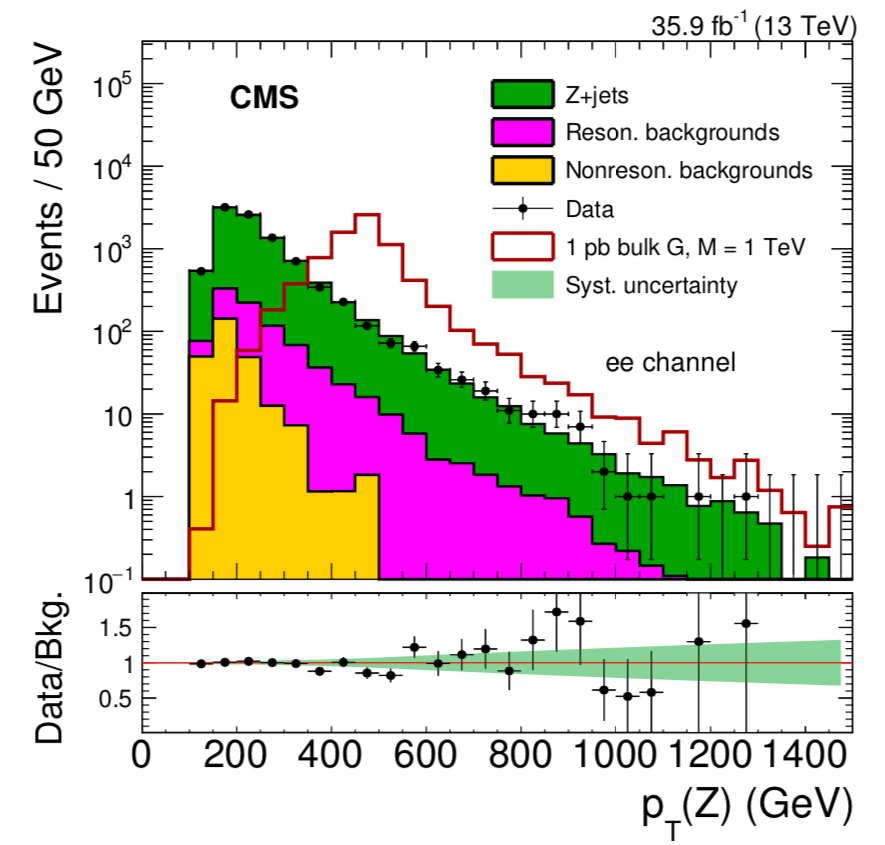
\includegraphics[width=0.49\linewidth]{figures/sys_elSRuncZpt.png}
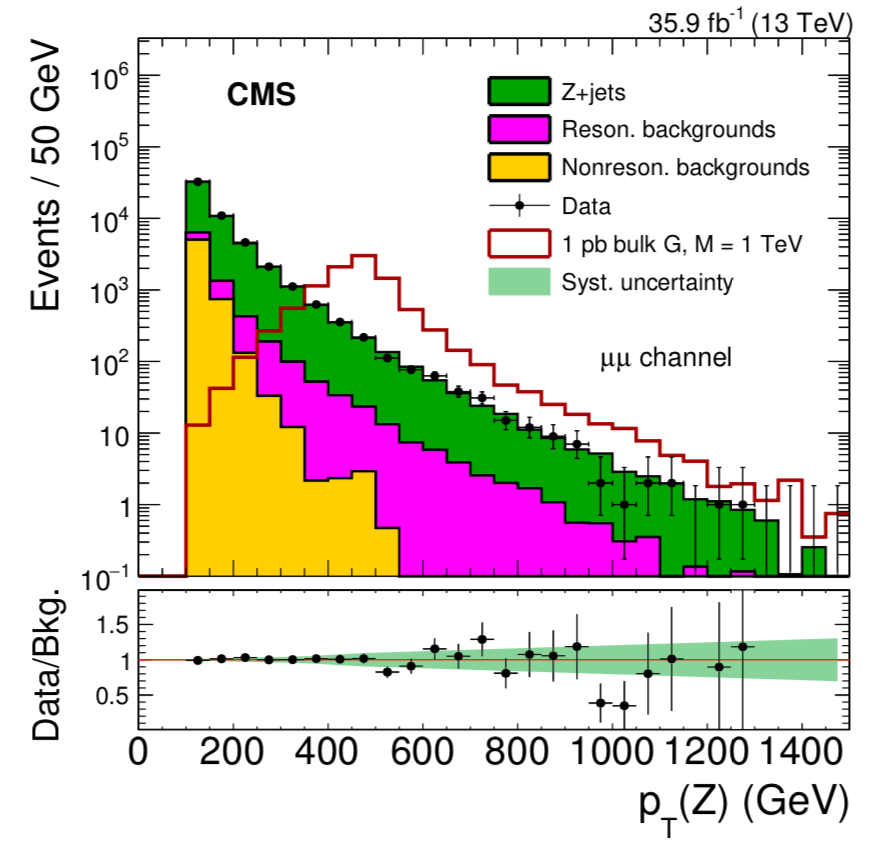
\includegraphics[width=0.49\linewidth]{figures/sys_muSRuncZpt.png}
\caption{$p_T ^Z$ for electron (left) and muon (right) channels comparing the data and background. The expected distribution for a zero width bulk graviton resonance with a mass of 1 TeV is also shown for a value of 1 pb for the product of cross section and branching fraction $\sigma(pp\rightarrow X\rightarrow ZZ)B(ZZ\rightarrow 2\ell 2\mu)$. The lower panels show the ratio of data to the prediction for the background. }
\label{fig:sys_uncZpt}
\end{center}
\end{figure}

\begin{figure}[htbp]
\begin{center}
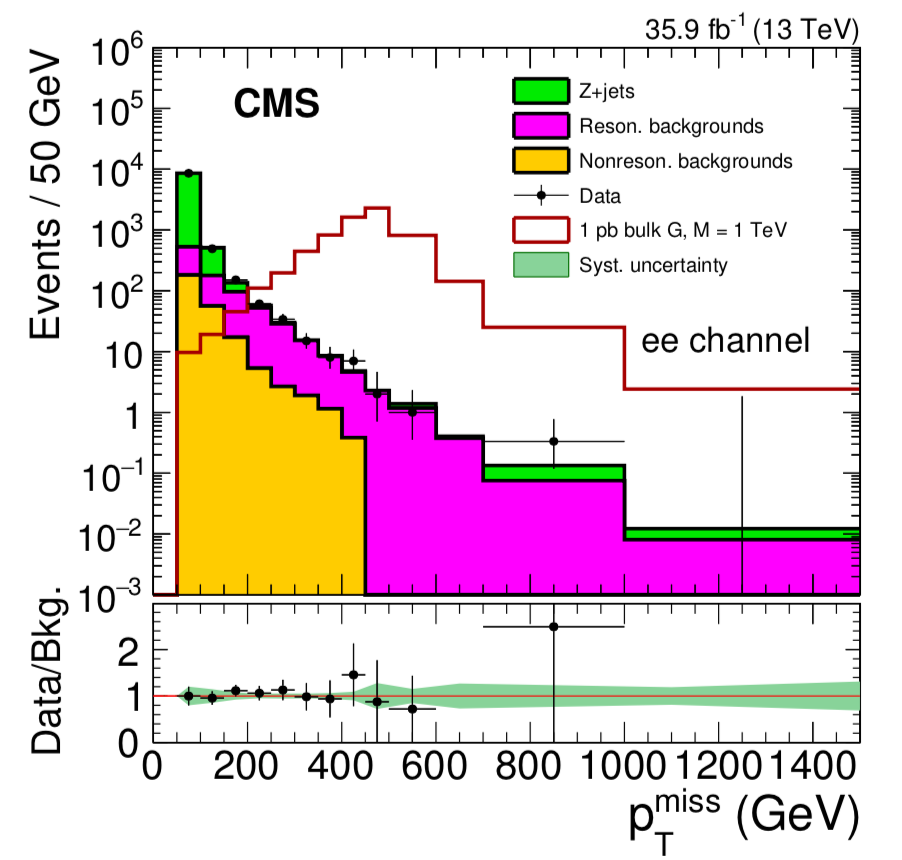
\includegraphics[width=0.49\linewidth]{figures/sys_elSRuncMET.png}
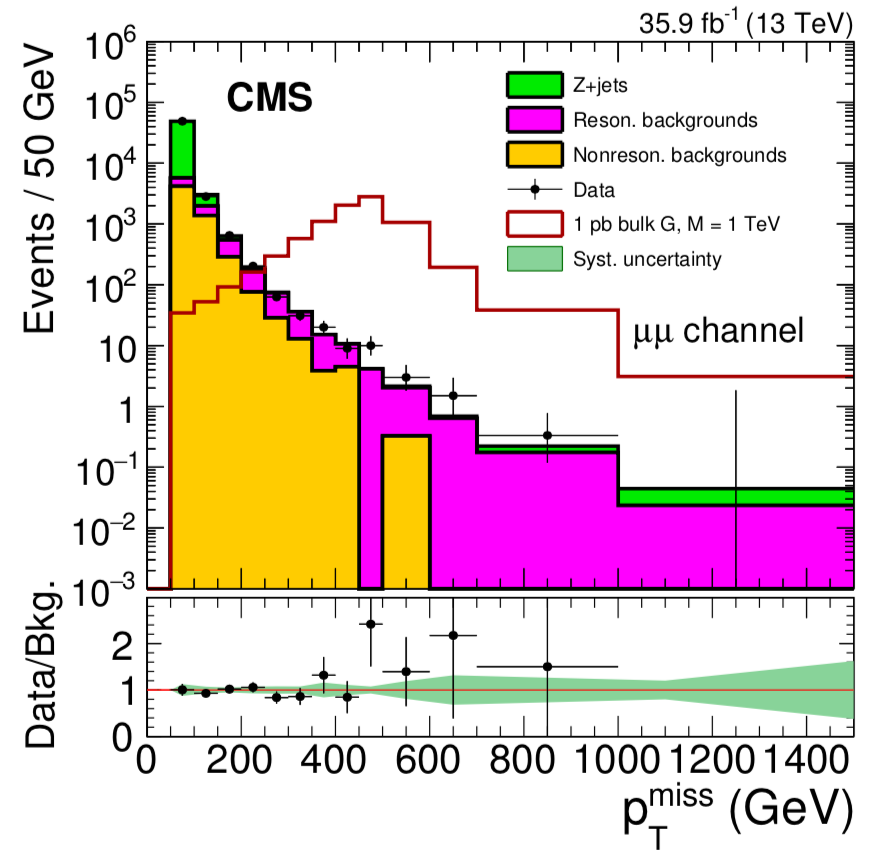
\includegraphics[width=0.49\linewidth]{figures/sys_muSRuncMET.png}
\caption{$p_T ^{miss}$ for electron (left) and muon (right) channels comparing the data and background. The expected distribution for a zero width bulk graviton resonance with a mass of 1 TeV is also shown for a value of 1 pb for the product of cross section and branching fraction $\sigma(pp\rightarrow X\rightarrow ZZ)B(ZZ\rightarrow 2\ell 2\mu)$. The lower panels show the ratio of data to the prediction for the background. }
\label{fig:sys_uncMET}
\end{center}
\end{figure}


\section{Results and Interpretation}
The $m_T$ distribution is used as the sensitive variable to search for a new resonance decaying to ZZ with the subsequent decay $ZZ\rightarrow 2\ell 2\nu$. The asymptotic approximation~\cite{sys_cls0} of the frequentist approach $CL_s$ technique~\cite{sys_cls1,sys_cls2,sys_cls3} is applied to determine the expected and observed upper limits for the possible signal strength at 95\% confidence level. The HiggsCombine Tool~\cite{sys_higgscombinetool} is used to obtain the limits. A binned shape analysis is applied considering the statistical uncertainties in the background modeling, and the following sources of systematic uncertaintiess are included by evaluating their corresponding effects on the $m_T$ distributions.
\begin{itemize}
\item HLT efficiency
\item lepton ID/Iso efficiency
\item QCD \& EW corrections for the resonance background
\item Z $p_T$ reweighting for the Zjets background
\item MET lepton/photon $p_T$
\item MET Jet energy resolution
\item MET unclustered-energy
\item MET Hadronic recoil 
\end{itemize}

Based on the $m_T$ spectrums of the systematics and background/signal, a binned likelihood simultaneous fit is performed to match the data better. Figure~\ref{fig:sys_uncMT} shows the $m_T$ distribution in the signal region after the background-only fit, with the background systematic uncertainties shown as the shaded band and data statistical uncertainty shown by the error bars. The observed distributions are in agreement with the SM background predictions.

\begin{figure}[htbp]
\begin{center}
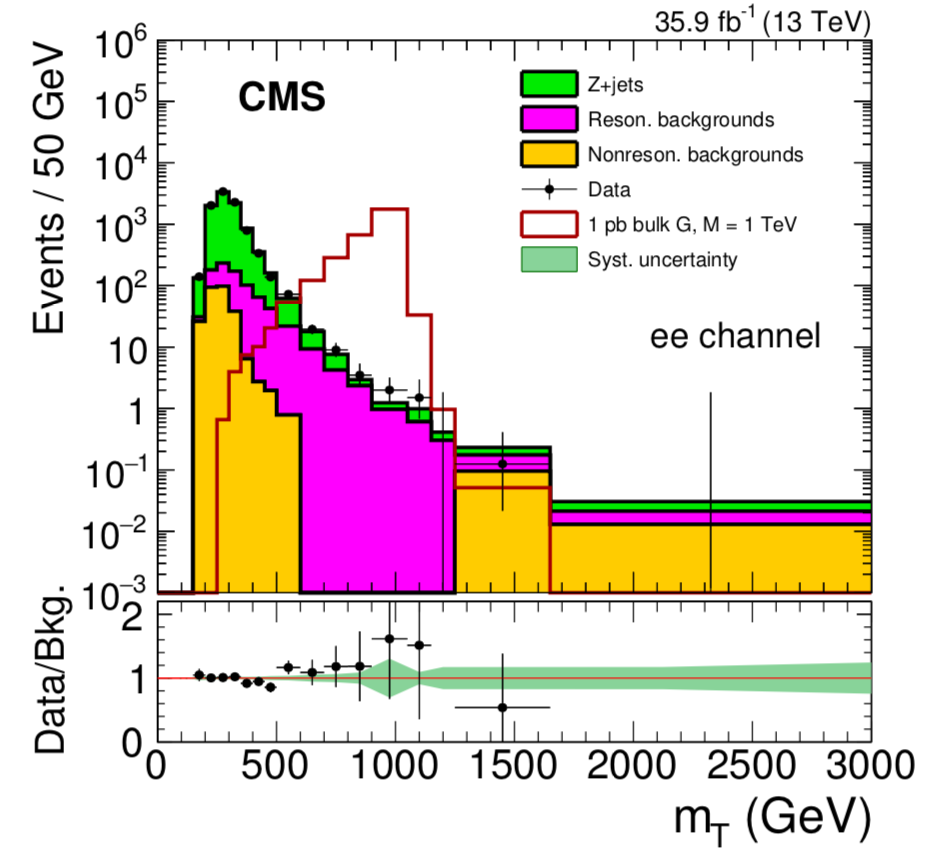
\includegraphics[width=0.49\linewidth]{figures/sys_elSRuncMT.png}
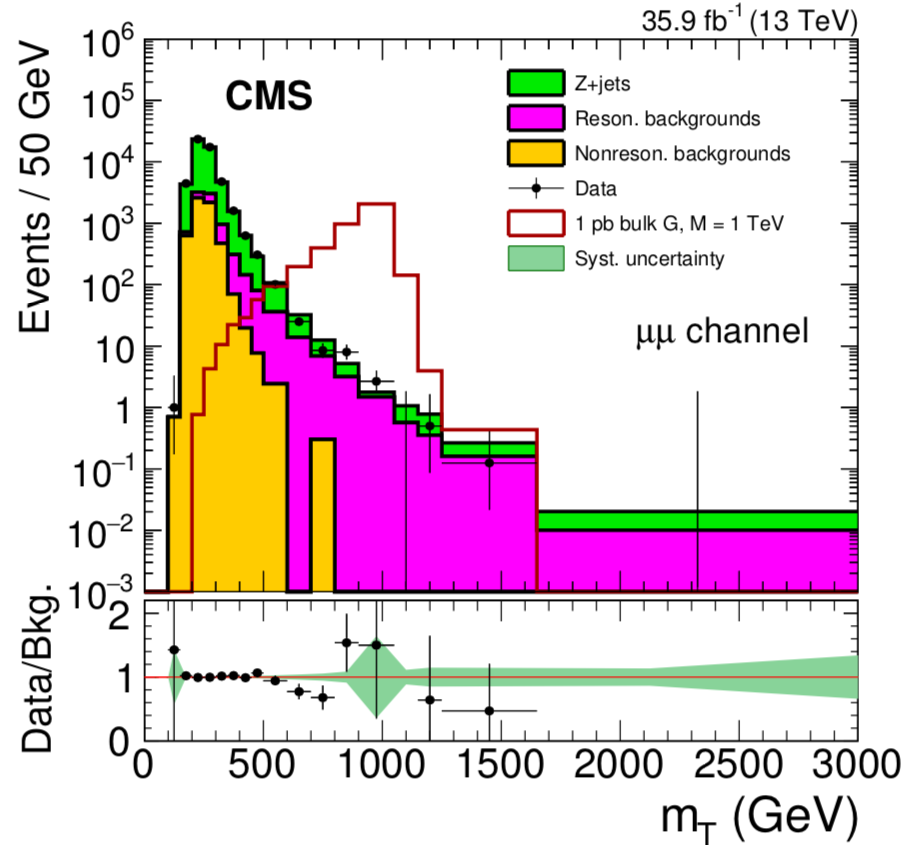
\includegraphics[width=0.49\linewidth]{figures/sys_muSRuncMT.png}
\caption{The $m_T$ distributions for electron (left) and muon (right) channels comparing the data and background, after fitting the background-only model to the data. The expected distribution for a zero width bulk graviton resonance with a mass of 1TeV is also shown for a value of 1pb for the product of branching fraction and cross section $\sigma(pp\rightarrow X\rightarrow ZZ)B(ZZ\rightarrow 2\ell 2\mu)$. The lower panels show the ratio of data to the prediction for the background.}
\label{fig:sys_uncMT}
\end{center}
\end{figure}

\vspace{0.3cm}
The expected upper limits are obtained from the modeled background and the signal, and the observed limits are then extracted combining the observed data after the simultaneous fit of background and signal for given signal hypotheses, for electron channel, muon channel and two channels combined. 

\vspace{0.3cm}
Figure~\ref{fig:sys_narrowlimits} shows the expected and observed upper limits on the product of the production cross section and the branching fraction for $X\rightarrow ZZ$ determined at the 95\% confidence level for the zero width benchmark model, electron and muon channels combined, shown with respect to the Graviton mass. Theorectical expectations of $\sigma(pp\rightarrow X\rightarrow ZZ)$ are also shown as a function of the Graviton mass, separately for $\tilde{k}=1.0,0.5,0.1$. The observed limits are within 2 standard deviations of expectations from the background-only model, therefore no evidence of new particle is observed. The hypothesis of $\tilde{k}=0.5$ can be excluded for masses below 800 GeV at 95\% CL, while the current data are not yet sensitive to the hypothesis of $\tilde{k}=0.1$. Figure~\ref{fig:sys_narrowlimitselmu} shows the limit plots for electron channel and muon channel separately.

\begin{figure}[htbp]
\begin{center}
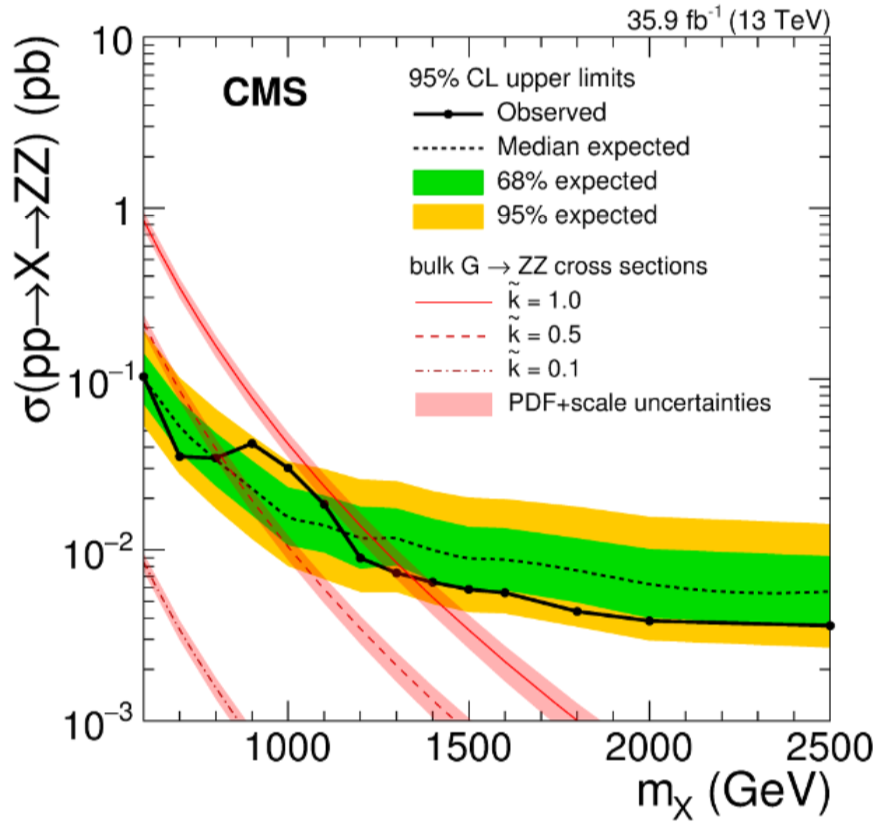
\includegraphics[width=0.9\linewidth]{figures/sys_narrowlimit.png}
\caption{Expected and observed limits on the product of cross section and branching fraction of the $pp\rightarrow G_{bulk}\rightarrow ZZ$ process, with zero-width assumption.}
\label{fig:sys_narrowlimits}
\end{center}
\end{figure}

\begin{figure}[htbp]
\begin{center}
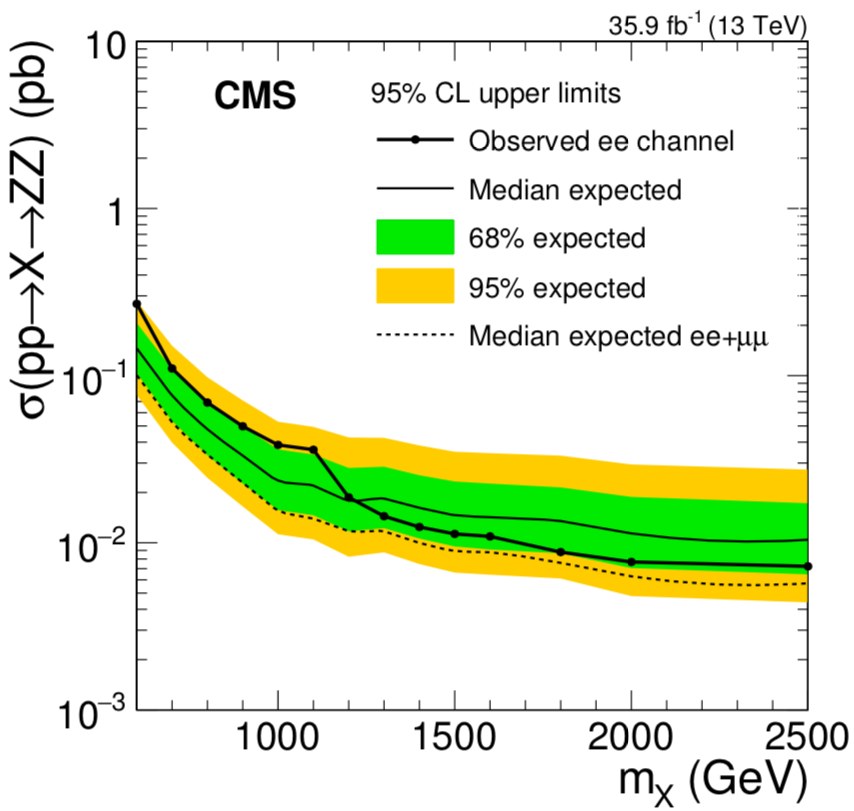
\includegraphics[width=0.49\linewidth]{figures/sys_narrowlimitsel.png}
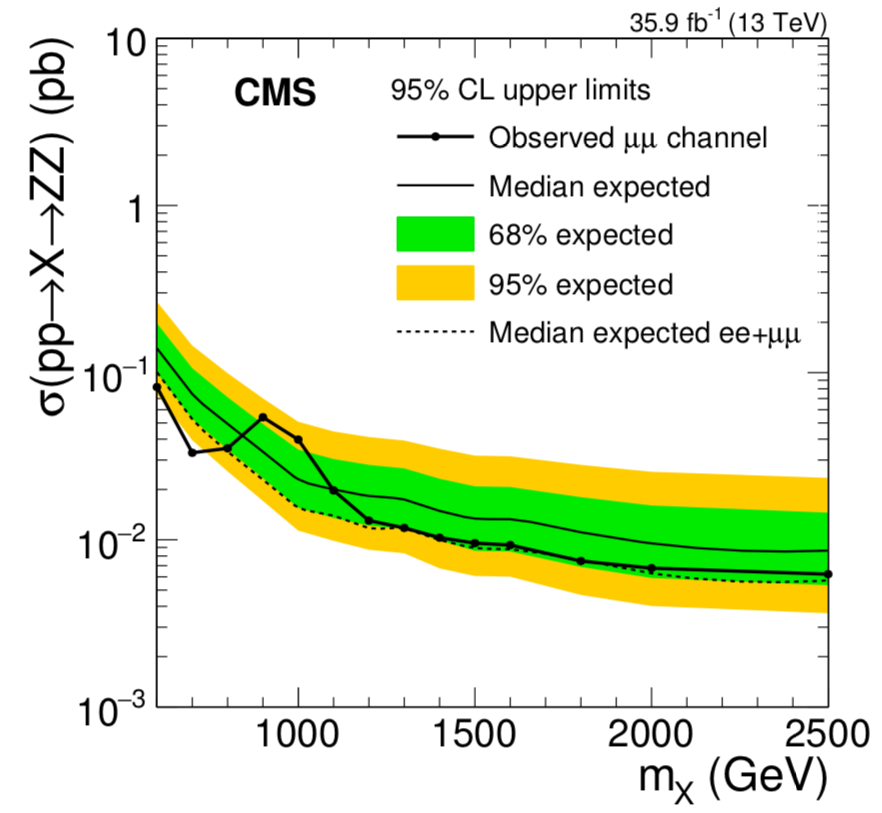
\includegraphics[width=0.49\linewidth]{figures/sys_narrowlimitsmu.png}
\caption{Expected and observed limits on the product of cross section and branching fraction of the $pp\rightarrow G_{bulk}\rightarrow ZZ$ process, with zero-width assumption, for the electron channel (left) and muon channel (right).}
\label{fig:sys_narrowlimitselmu}
\end{center}
\end{figure}

\vspace{0.3cm}
The analysis of the upper limits is also performed on the more general wide width version of the bulk graviton model. And the production initial state is set to be either a gluon–gluon fusion or $q\bar{q}$ annihilation process. The width of the resonance is set to be 0/10\%/20\%/30\% of the resonance mass. Figure~\ref{fig:sys_ggqqlimits} shows the limits for the wide width model.

\begin{figure}[htbp]
\begin{center}
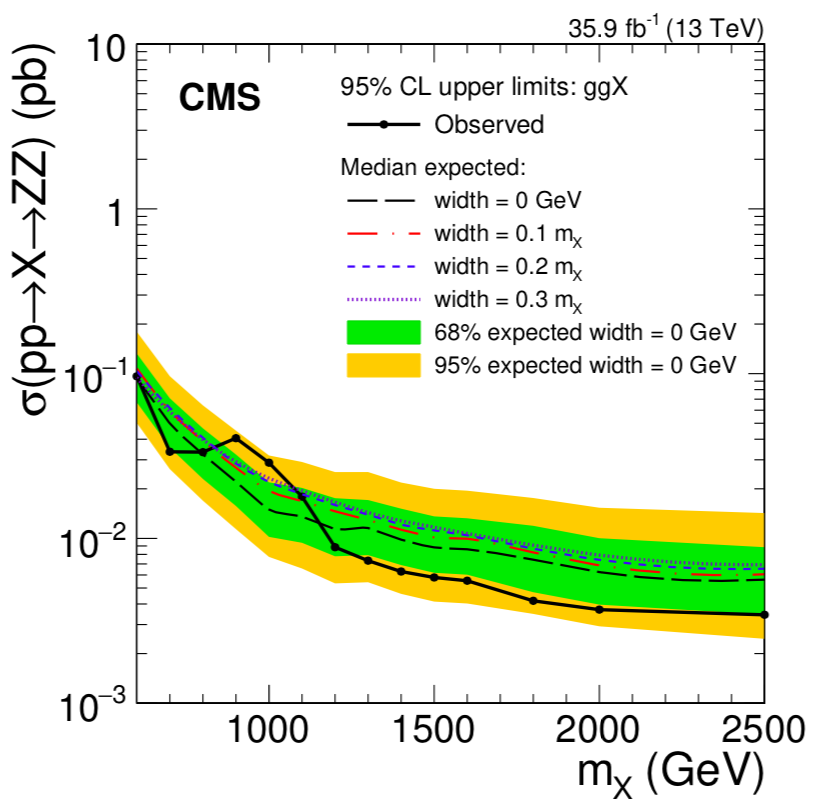
\includegraphics[width=0.49\linewidth]{figures/sys_gglimits.png}
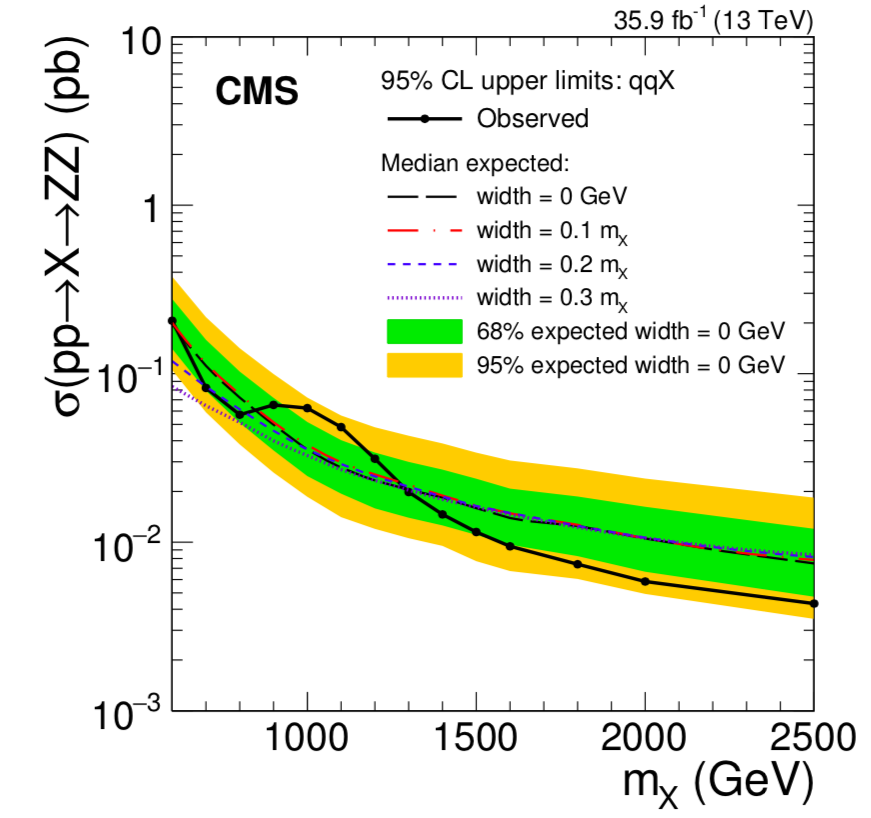
\includegraphics[width=0.49\linewidth]{figures/sys_qqlimits.png}
\caption{Expected and observed limits on the product of cross section and branching fraction of the $pp\rightarrow G_{bulk}\rightarrow ZZ$ process, electron channel and muon channel combined, with signal width being 0/10\%/20\%/30\% of the resonance mass, for gluon–gluon fusion production (left) and $q\bar{q}$ annihilation production (right).}
\label{fig:sys_ggqqlimits}
\end{center}
\end{figure}

\vspace{0.3cm}
Considering that gluon–gluon fusion is the dominant production for the Bulk Graviton, the zero-width gluon–gluon fusion limit plot looks very similar to Figure~\ref{fig:sys_narrowlimits}. The $q\bar{q}$ production limits differ due to the spin and parity effects~\cite{sys_resoproduction}. Figure~\ref{fig:sys_ggqqdiff} shows the normalized $m_T$ distribution of the gluon–gluon production and $q\bar{q}$ production, as well as combined production. The $m_T$ spectrum of the $q\bar{q}$ production is much less strongly peaked than gluon–gluon fusion, which causes the expected and observed cross-section upper limit of the $q\bar{q}$ production to be higher.
\begin{figure}[htbp]
\begin{center}
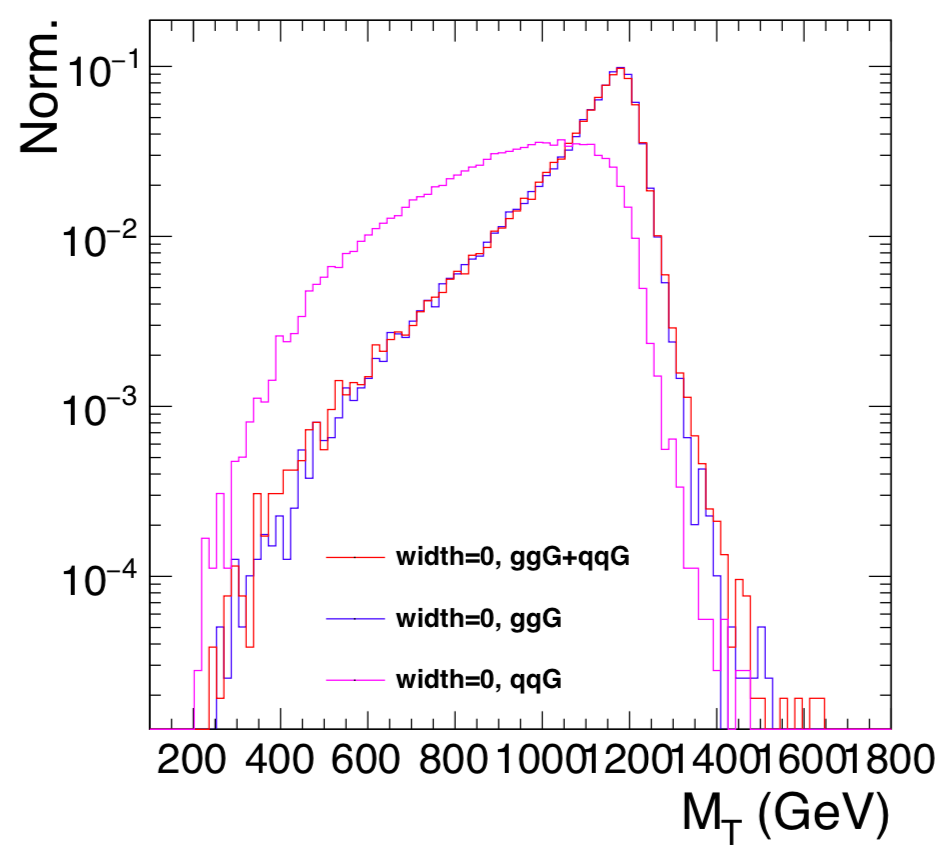
\includegraphics[width=0.9\linewidth]{figures/sys_ggqqdiff.png}
\caption{The $m_T$ distributions for spin-2 resonance signal samples for gluon fusion production and $q\bar{q}$ production.}
\label{fig:sys_ggqqdiff}
\end{center}
\end{figure}
